% Options for packages loaded elsewhere
\PassOptionsToPackage{unicode}{hyperref}
\PassOptionsToPackage{hyphens}{url}
\PassOptionsToPackage{dvipsnames,svgnames*,x11names*}{xcolor}
%
\documentclass[
  12pt,
  dvipsnames,enabledeprecatedfontcommands]{scrartcl}
\usepackage{amsmath,amssymb}
\usepackage{lmodern}
\usepackage{ifxetex,ifluatex}
\ifnum 0\ifxetex 1\fi\ifluatex 1\fi=0 % if pdftex
  \usepackage[T1]{fontenc}
  \usepackage[utf8]{inputenc}
  \usepackage{textcomp} % provide euro and other symbols
\else % if luatex or xetex
  \usepackage{unicode-math}
  \defaultfontfeatures{Scale=MatchLowercase}
  \defaultfontfeatures[\rmfamily]{Ligatures=TeX,Scale=1}
\fi
% Use upquote if available, for straight quotes in verbatim environments
\IfFileExists{upquote.sty}{\usepackage{upquote}}{}
\IfFileExists{microtype.sty}{% use microtype if available
  \usepackage[]{microtype}
  \UseMicrotypeSet[protrusion]{basicmath} % disable protrusion for tt fonts
}{}
\makeatletter
\@ifundefined{KOMAClassName}{% if non-KOMA class
  \IfFileExists{parskip.sty}{%
    \usepackage{parskip}
  }{% else
    \setlength{\parindent}{0pt}
    \setlength{\parskip}{6pt plus 2pt minus 1pt}}
}{% if KOMA class
  \KOMAoptions{parskip=half}}
\makeatother
\usepackage{xcolor}
\IfFileExists{xurl.sty}{\usepackage{xurl}}{} % add URL line breaks if available
\IfFileExists{bookmark.sty}{\usepackage{bookmark}}{\usepackage{hyperref}}
\hypersetup{
  colorlinks=true,
  linkcolor=Maroon,
  filecolor=Maroon,
  citecolor=Blue,
  urlcolor=blue,
  pdfcreator={LaTeX via pandoc}}
\urlstyle{same} % disable monospaced font for URLs
\usepackage{graphicx}
\makeatletter
\def\maxwidth{\ifdim\Gin@nat@width>\linewidth\linewidth\else\Gin@nat@width\fi}
\def\maxheight{\ifdim\Gin@nat@height>\textheight\textheight\else\Gin@nat@height\fi}
\makeatother
% Scale images if necessary, so that they will not overflow the page
% margins by default, and it is still possible to overwrite the defaults
% using explicit options in \includegraphics[width, height, ...]{}
\setkeys{Gin}{width=\maxwidth,height=\maxheight,keepaspectratio}
% Set default figure placement to htbp
\makeatletter
\def\fps@figure{htbp}
\makeatother
\setlength{\emergencystretch}{3em} % prevent overfull lines
\providecommand{\tightlist}{%
  \setlength{\itemsep}{0pt}\setlength{\parskip}{0pt}}
\setcounter{secnumdepth}{5}
%\documentclass{article}

% %packages
 \usepackage{booktabs}

\usepackage{multirow}
\usepackage{multicol}
\usepackage{subcaption}
\usepackage{graphicx}
\usepackage{longtable}
\usepackage{ragged2e}
\usepackage{etex}
%\usepackage{yfonts}
\usepackage{marvosym}
\usepackage[notextcomp]{kpfonts}
\usepackage{nicefrac}
\newcommand*{\QED}{\hfill \footnotesize {\sc Q.e.d.}}
\usepackage{floatrow}



\usepackage[textsize=scriptsize, textwidth = 1.5cm]{todonotes}
%\linespread{1.5}


\setlength{\parindent}{10pt}
\setlength{\parskip}{1pt}


%language
\usepackage{times}
\usepackage{t1enc}
%\usepackage[utf8x]{inputenc}
%\usepackage[polish]{babel}
%\usepackage{polski}

\usepackage{mathptmx}
\usepackage[scaled=0.88]{helvet}


%AMS
\usepackage{amsfonts}
\usepackage{amssymb}
\usepackage{amsthm}
\usepackage{amsmath}
\usepackage{mathtools}

\usepackage{geometry}
 \geometry{a4paper,left=35mm,top=20mm,bottom = 20mm, right = 35mm}


%environments
\newtheorem{fact}{Fact}



%abbreviations
\newcommand{\ra}{\rangle}
\newcommand{\la}{\langle}
\newcommand{\n}{\neg}
\newcommand{\et}{\wedge}
\newcommand{\jt}{\rightarrow}
\newcommand{\ko}[1]{\forall  #1\,}
\newcommand{\ro}{\leftrightarrow}
\newcommand{\exi}[1]{\exists\, {_{#1}}}
\newcommand{\pr}[1]{\mathsf{P}(#1)}
\newcommand{\cost}{\mathsf{cost}}


\newcommand{\odds}{\mathsf{Odds}}
\newcommand{\ind}{\mathsf{Ind}}
\newcommand{\nf}[2]{\nicefrac{#1\,}{#2}}
\newcommand{\R}[1]{\texttt{#1}}
\newcommand{\prr}[1]{\mbox{$\mathtt{P}_{prior}(#1)$}}
\newcommand{\prp}[1]{\mbox{$\mathtt{P}_{posterior}(#1)$}}



\newtheorem{q}{\color{blue}Question}
\newtheorem{lemma}{Lemma}
\newtheorem{theorem}{Theorem}



%technical intermezzo
%---------------------

\newcommand{\intermezzoa}{
	\begin{minipage}[c]{13cm}
	\begin{center}\rule{10cm}{0.4pt}



	\tiny{\sc Optional Content Starts}
	
	\vspace{-1mm}
	
	\rule{10cm}{0.4pt}\end{center}
	\end{minipage}\nopagebreak 
	}


\newcommand{\intermezzob}{\nopagebreak 
	\begin{minipage}[c]{13cm}
	\begin{center}\rule{10cm}{0.4pt}

	\tiny{\sc Optional Content Ends}
	
	\vspace{-1mm}
	
	\rule{10cm}{0.4pt}\end{center}
	\end{minipage}
	}
%--------------------

\DeclareUnicodeCharacter{0301}{*************************************}




















\newtheorem*{reply*}{Reply}
\usepackage{enumitem}
\newcommand{\question}[1]{\begin{enumerate}[resume,leftmargin=0cm,labelsep=0cm,align=left]
\item #1
\end{enumerate}}

\usepackage{float}

% \setbeamertemplate{blocks}[rounded][shadow=true]
% \setbeamertemplate{itemize items}[ball]
% \AtBeginPart{}
% \AtBeginSection{}
% \AtBeginSubsection{}
% \AtBeginSubsubsection{}
% \setlength{\emergencystretch}{0em}
% \setlength{\parskip}{0pt}






\usepackage[authoryear]{natbib}

%\bibliographystyle{apalike}
\usepackage{booktabs}
\usepackage{longtable}
\usepackage{array}
\usepackage{multirow}
\usepackage{wrapfig}
\usepackage{float}
\usepackage{colortbl}
\usepackage{pdflscape}
\usepackage{tabu}
\usepackage{threeparttable}
\usepackage{threeparttablex}
\usepackage[normalem]{ulem}
\usepackage{makecell}
\usepackage{xcolor}
\ifluatex
  \usepackage{selnolig}  % disable illegal ligatures
\fi
\newlength{\cslhangindent}
\setlength{\cslhangindent}{1.5em}
\newlength{\csllabelwidth}
\setlength{\csllabelwidth}{3em}
\newenvironment{CSLReferences}[2] % #1 hanging-ident, #2 entry spacing
 {% don't indent paragraphs
  \setlength{\parindent}{0pt}
  % turn on hanging indent if param 1 is 1
  \ifodd #1 \everypar{\setlength{\hangindent}{\cslhangindent}}\ignorespaces\fi
  % set entry spacing
  \ifnum #2 > 0
  \setlength{\parskip}{#2\baselineskip}
  \fi
 }%
 {}
\usepackage{calc}
\newcommand{\CSLBlock}[1]{#1\hfill\break}
\newcommand{\CSLLeftMargin}[1]{\parbox[t]{\csllabelwidth}{#1}}
\newcommand{\CSLRightInline}[1]{\parbox[t]{\linewidth - \csllabelwidth}{#1}\break}
\newcommand{\CSLIndent}[1]{\hspace{\cslhangindent}#1}

\author{}
\date{\vspace{-2.5em}}

\begin{document}

\begin{center}
\large \textbf{Taking uncertainty seriously}

\textbf{A  Bayesian approach to  word embedding bias estimation }
\end{center}

\vspace{1mm}

A considerable amount of literature exists on bias detection and
mitigation in NLP models, especially word embeddings, which represent
words as vectors of real numbers (see e.g. {[}1{]} and {[}4{]} and
references therein). The most common methods used compare cosine
similarity or distance between words from protected groups and
attributes that are considered to be stereotypical or harmful in some
way. Many of them rely on pre-averaging, which we find problematic ---
two such methods will be in our focus. We will argue that the existing
measures of bias by pre-averaging oversimplify the picture and lead to
false confidence. Our simulation results show that the mainstream
interpretations are too hasty. Our Bayesian analysis with proper control
groups suggests that (1) the word lists in use are too short, (2)
associated and different groups behave similarly, which undermines the
semantic interpretation of cosine similarity, and (3) our analysis at
different levels of generality shows that there is more variety than one
may initially think.

In one well-known approach, {[}2{]} proposed the Word Embedding
Association Test (WEAT). The idea is that the measure of biases between
two sets of target words, \(X\) and \(Y\), (we call them protected
words) should be quantified in terms of the cosine similarity between
the protected words and attribute words coming from two sets of
stereotype attribute words, \(A\) and \(B\) (we'll call them
attributes). For instance, \(X\) might be a set of male names, \(Y\) a
set of female names, \(A\) might contain stereotypically male-related
career words, and \(B\) stereotypically female-related family words.
WEAT is a modification of the Implicit Association Test (IAT) {[}7{]}
used in psychology and uses almost the same word sets, allowing for a
\emph{prima facie} sensible comparison with bias in humans. The
association difference for a term \(t\) is \(s(t,A,B)\), and the effect
size is computed by normalizing the difference in means as follows
(\(f\) is a similarity measure, such as cosine similarity):

\vspace{-3mm}

\footnotesize \begin{align}
\mathsf{s}(t,A,B)  = \frac{\sum_{a\in A}f(t,a)}{\vert A\vert} - \frac{\sum_{b\in B}f(t,b)}{\vert B\vert}
& \,\,\,\,\,\,\,\,\,\,\,\,\,\,\,\,\,
\mathsf{bias}(A,B)  = \frac{
\mu(\{s(x,A,B)\}_{x\in X}) -\mu(\{s(y,A,B)\}_{y\in Y}) 
}{
\sigma(\{s(w,A,B)\}_{w\in X\cup Y})
} \tag{WEAT}
\end{align} \normalsize \noindent {[}2{]} show that significant
biases---thus measured--- similar to the ones discovered by IAT can be
discovered in word embeddings. {[}5{]} extend the methodology to a
multilingual and cross-lingual setting; a similar methodology is
employed by {[}3{]}, who use word embeddings trained on corpora from
different decades. {[}6{]} modify WEAT to a multi-class setting,
introducing Mean Average Cosine (MAC) similarity distance as a measure
of bias. Let \(T = \{t_1, \dots, t_k\}\) be a class of protected word
embeddings, and let each \(A_j\in A\) be a set of attributes
stereotypically associated with a protected word). Then:

\vspace{-2mm}

\footnotesize

\begin{align}
\mathsf{S}(t_i, A_j)  = \frac{1}{\vert A_j\vert}\sum_{a\in A_j}\mathsf{cos}(t,a) & \,\,\,\,\,\,\,\,\,\,\,\,\,\,\,\,\,\,\,\,\,\,\,\,\,
\mathsf{MAC}(T,A)  = \frac{1}{\vert T \vert \,\vert A\vert}\sum_{t_i \in T }\sum_{A_j \in A} S(t_i,A_j) \tag{MAC}
\end{align} \normalsize  \noindent That is, for each protected word and
each attribute class, they first take the mean for this protected word
and all attributes in a given attribute class, and then they take the
mean of thus obtained means for all the protected words.

Such methods are statistically problematic. Two issues, specific to
{[}6{]}, are that (i) no distinction is made based on whether a class of
attributes is stereotypically associated with a given protected word or
with a different protected word, and (ii) no re-scaling by standard
deviation (typical in effect size measures such as Cohen's \(d\)) is
used, so MAC is not a good measure of effect size. A more general
problem, is that all the authors ignore the step of comparing their
results with control groups, especially control groups of
stereotype-neutral human attributes. That such a move is important is
suggested for instance by Figure 1 prepared using the original word list
for religion-related protected words extended with control attributes,
where such human attributes are also closer to protected classes than
neutral non-human words.

Another serious problem is that all the authors calculate means of means
and run statistical tests on sets of means. Unfortunately, by
pre-averaging the data they throw away information about sample sizes,
and they remove variation, and so pre-averaging tends to manufacture
false confidence.

To illustrate, let's employ the formulas used by {[}2{]} in a simple
simulation. All such approaches come up with rather short lists of
protected words and rather short lists of stereotypical attributes.
Clearly, these are not complete list. So let's treat them as samples
from richer pools of stereotypical predicates and let's take the
uncertainty and variation involved seriously.

\begin{center}
\begin{tabular}{cccccc}\toprule
$X$ to $A$  & $X$ to $B$ & $Y$ to $A$ & $Y$ to $B$ & $\sigma$  & WEAT \\
\midrule
0 & 0 & 0 & 0 & 0.05 & 1.82 \\
0 & 0 & 0 & 0 & 0.001 & -1.93\\
.1 & 0 & 0 & .1 & 0.05 & 1.49 \\
.1 & 0 & 0 & .1 & .1 & 1.22\\
\bottomrule
\end{tabular}
\end{center}

To illustrate, we have randomly drawn protected classes,
\(X=\{t_1,t_2\}\) and \(Y=\{t_3,t_4\}\), and two five-element attribute
sets \(A\) and \(B\). One simulation draws normally distributed values
for two situations in which the underlying mean similarities are in fact
equal to zero, in two other cases the means are different, with a range
of choices of common standard deviation across the cases (see the
table). The following observations are worthwhile. For points randomly
drawn from distributions where there is no difference in means the
calculated effect size can easily be 1.82, whereas the largest effect
size reported by by Caliskan is 1.81. For samples from distributions
where the means are different, the (absolute) effect sizes can easily be
lower than in the first two simulations. Moreover, 10k simulations with
more realistic word list sizes (normal distributions with equal means,
standard deviation=0.08, 16 protected words and 16 predicates) show that
high scores are easy to get even if there is no difference in the
generating model (Figure 2, code available upon request). This indicates
that the low p-value reported in the papers are highly misleading.

To improve on the situation, we build Bayesian models to estimate the
biases involved using the raw data points, actually using control
groups, distinguishing the connection types, and taking the uncertainty
involved seriously. For the general impact of being associated, we build
models using Hamiltonian Monte Carlo (STAN) according to the following
specification (linear categorical model and the priors):

\footnotesize

\vspace{-5mm}

\begin{align}
cosineDistance_i  & \sim dnorm(\mu_i, \sigma) &
\mu_i & = m_{pw} + co_{con} \tag{Model}\\
m_{pw} & \sim dnorm(1,.5)  & 
co_{con} & \sim dnorm(0,1)  \,\,\,\,\,
 & \sigma  \sim  dcauchy(0,1) \tag{Priors}
\end{align} \normalsize 

\vspace{-2mm}

\noindent That is, given a protected word we assume its cosine distance
to attributes from a given group is normally distributed around a mean,
which is determined by the mean assigned to this protected word and by
the connection type of that group of attributes (stereotypically
associated/ associated with a different predicate/neutral human
attribute/random word), and we use weak regularizing priors for the
parameters. The task of the model is to estimate the mean for a given
protected word and the coefficients of change in that mean corresponding
to different connection types.

The resulting coefficients for the religion dataset based on Reddit
embeddings are in Figure 5. While there is some difference in the means,
the 89\% highest posterior density invervals are quite wide and include
0s for all the coefficients. Then, motivated by large differences
between the states of different protected words, we build bayesian
models with separate coefficients for protected classes, with analogous
regularizing priors. The results for the religion dataset based on
Reddit embeddings are in Figure 6.

We build analogous models for other topic groups (race, gender), and
different embeddings (we use three embeddings:
GoogleNews-vectors-negative300, and Reddit Corpus, and the hard-debiased
Reddit embedding used by {[}6{]}). The general conclusion is that from
this bayesian perpective the situation is much less obvious. The word
list sizes are small, sample sizes are small, and so posterior density
intervals are wide. Some stronger bias can be discerned in the gender
case. Moreover, sometimes the differences between associated, different
and human, are not very impressive. The cost of debiasing turns out
sometimes to be that neutral human predicates get closer to protected
classes (in religion), change in gender after debiasing is really minor
with zero still out of HPDI range, and debiasing improvement for race is
a small improvement achieved at the price of moving neutral terms closer
to protected words (there is no space to include these results in this
abstract).

The bottom line is that if we want to take bias seriously, so should we
approach the uncertainty involved in our estimations. There is no
replacement for proper statistical evaluation that does not discard
information about the uncertaintly involved, larger word lists are
needed, and visualisation of the results for particular protected
classes provides much better guidance than chasing a single metric based
on a means of means.

\pagebreak

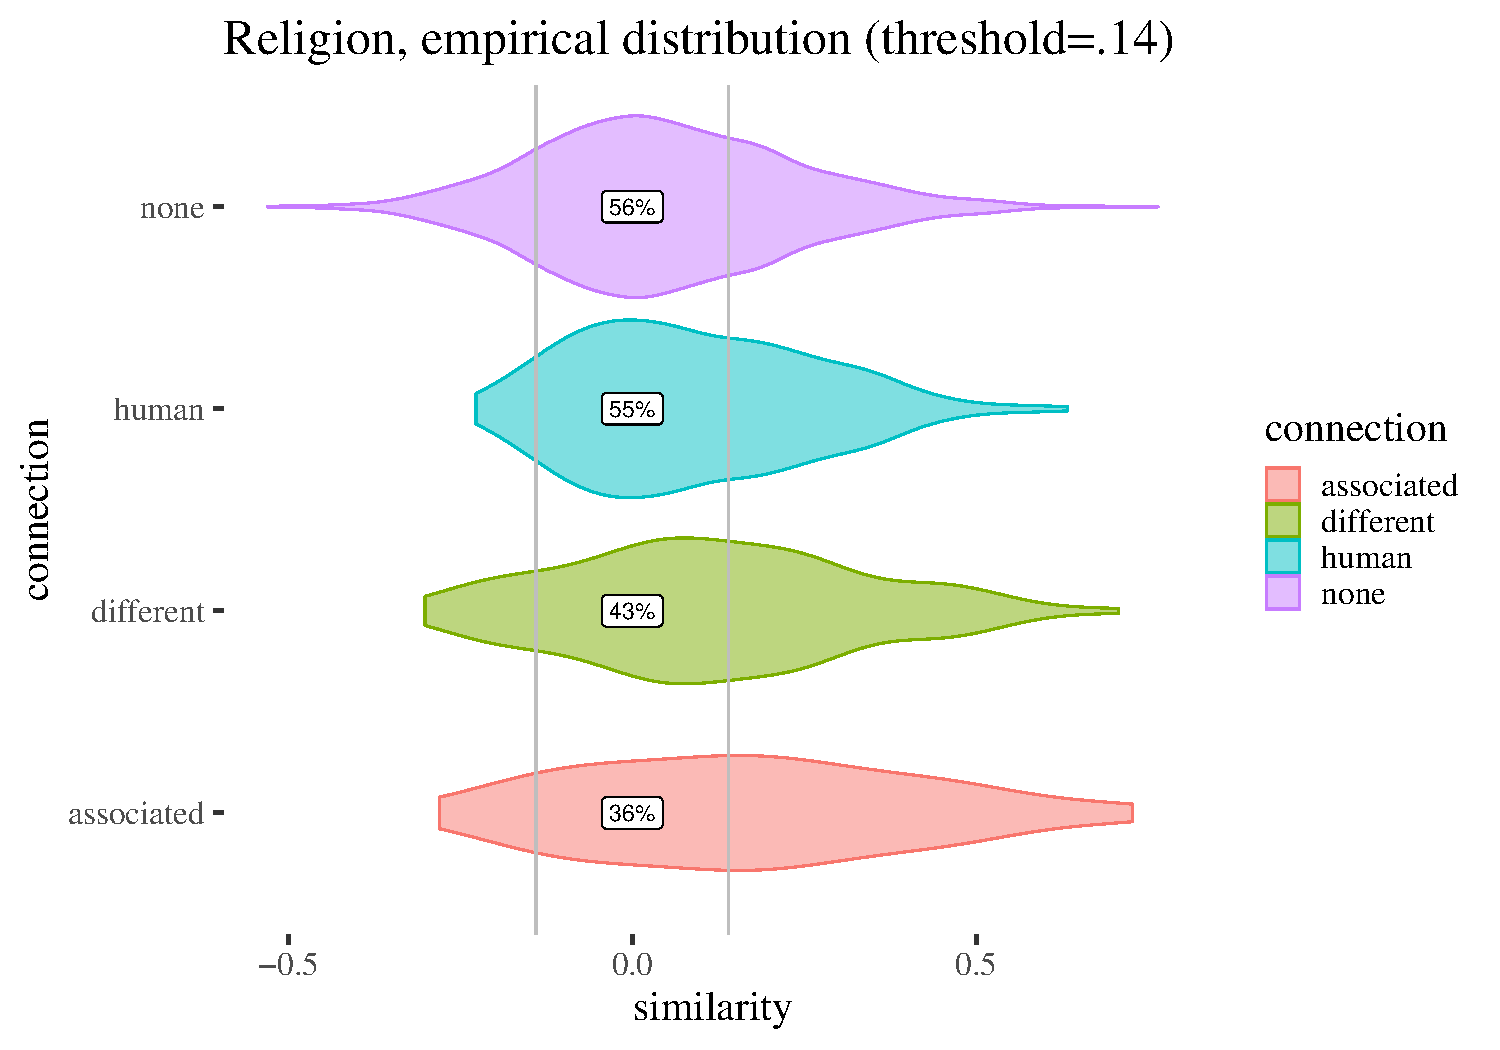
\includegraphics[width=8cm]{violinReligion.pdf}
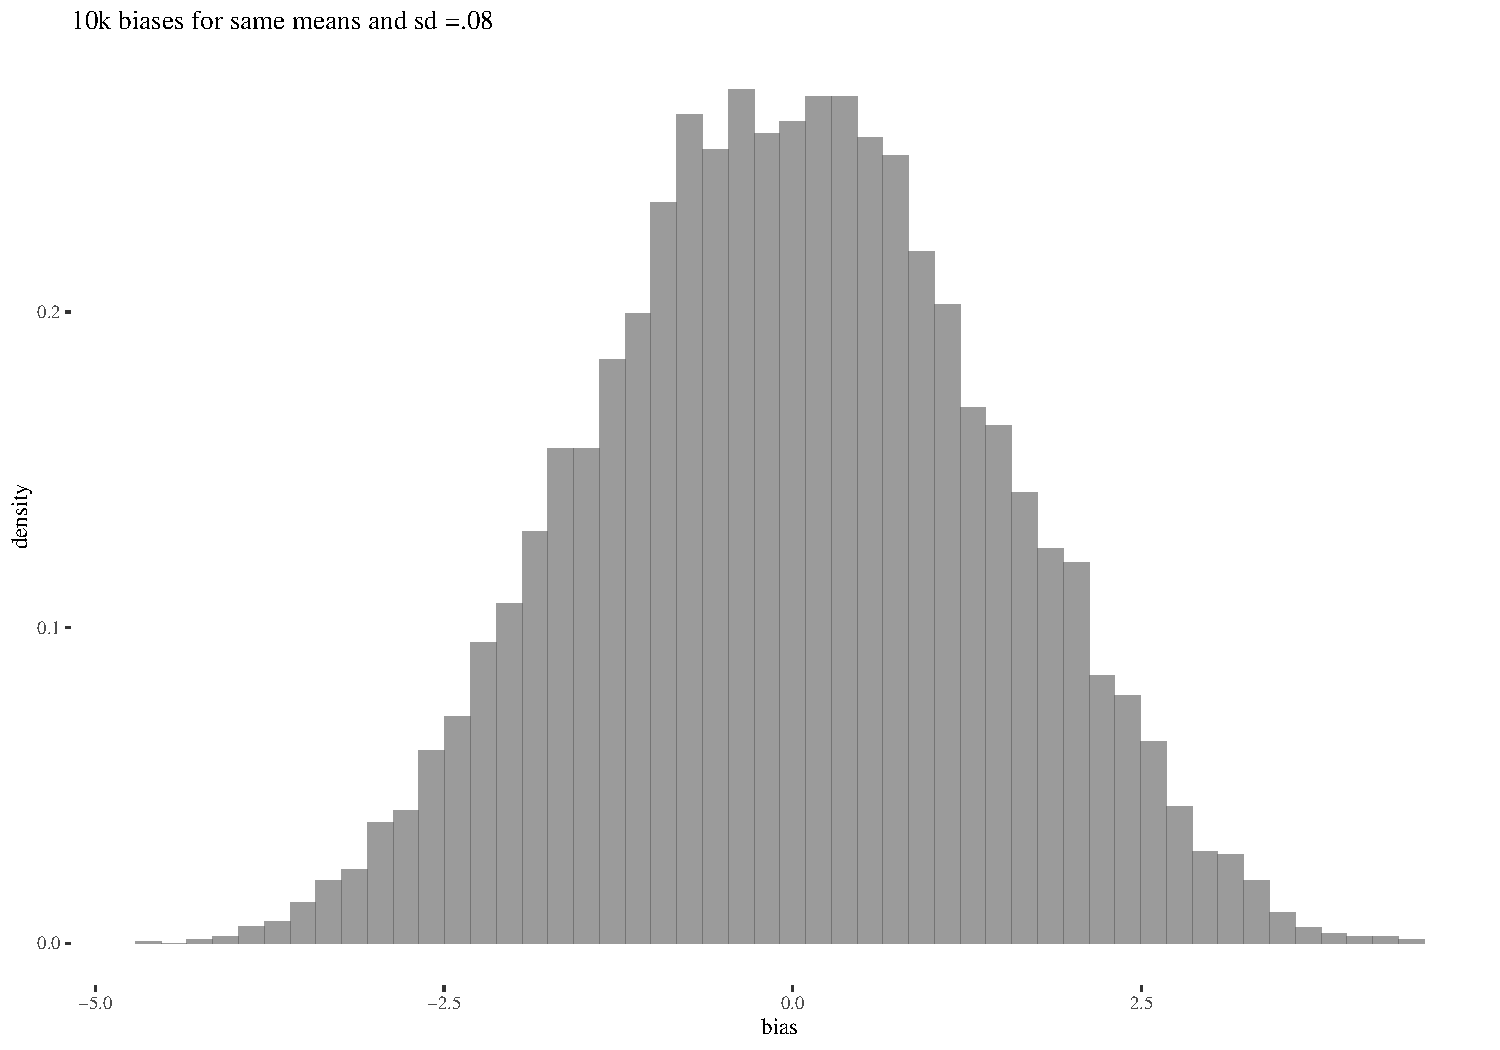
\includegraphics[width=8cm]{simulations.pdf}

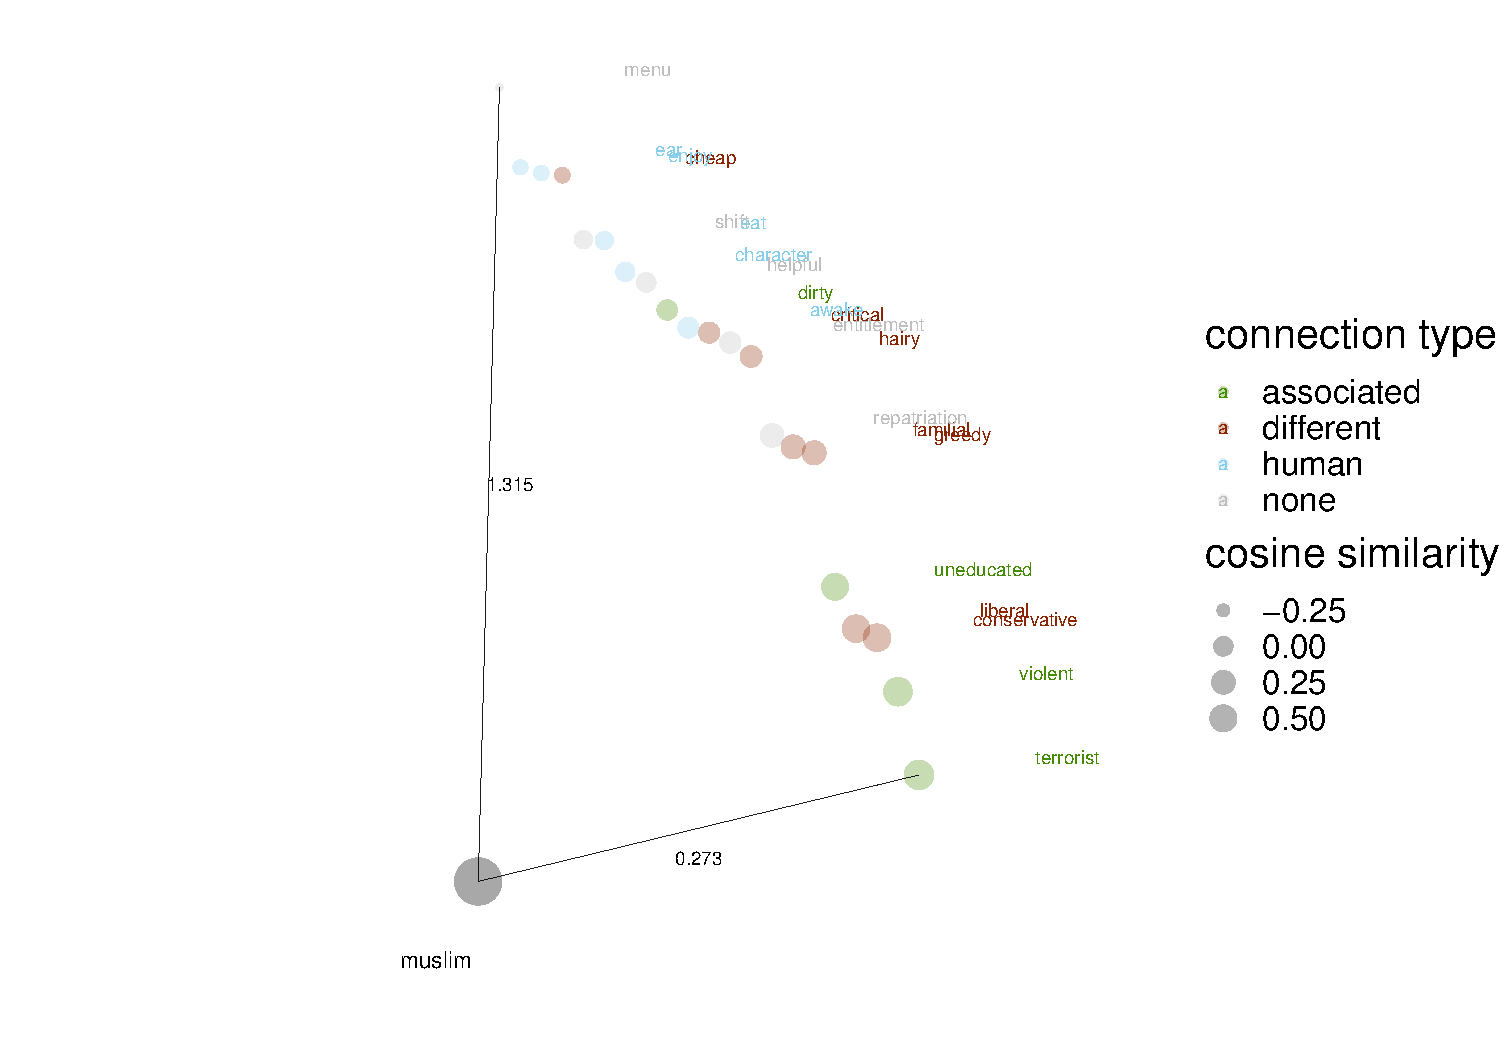
\includegraphics[width=8cm]{muslim.pdf}
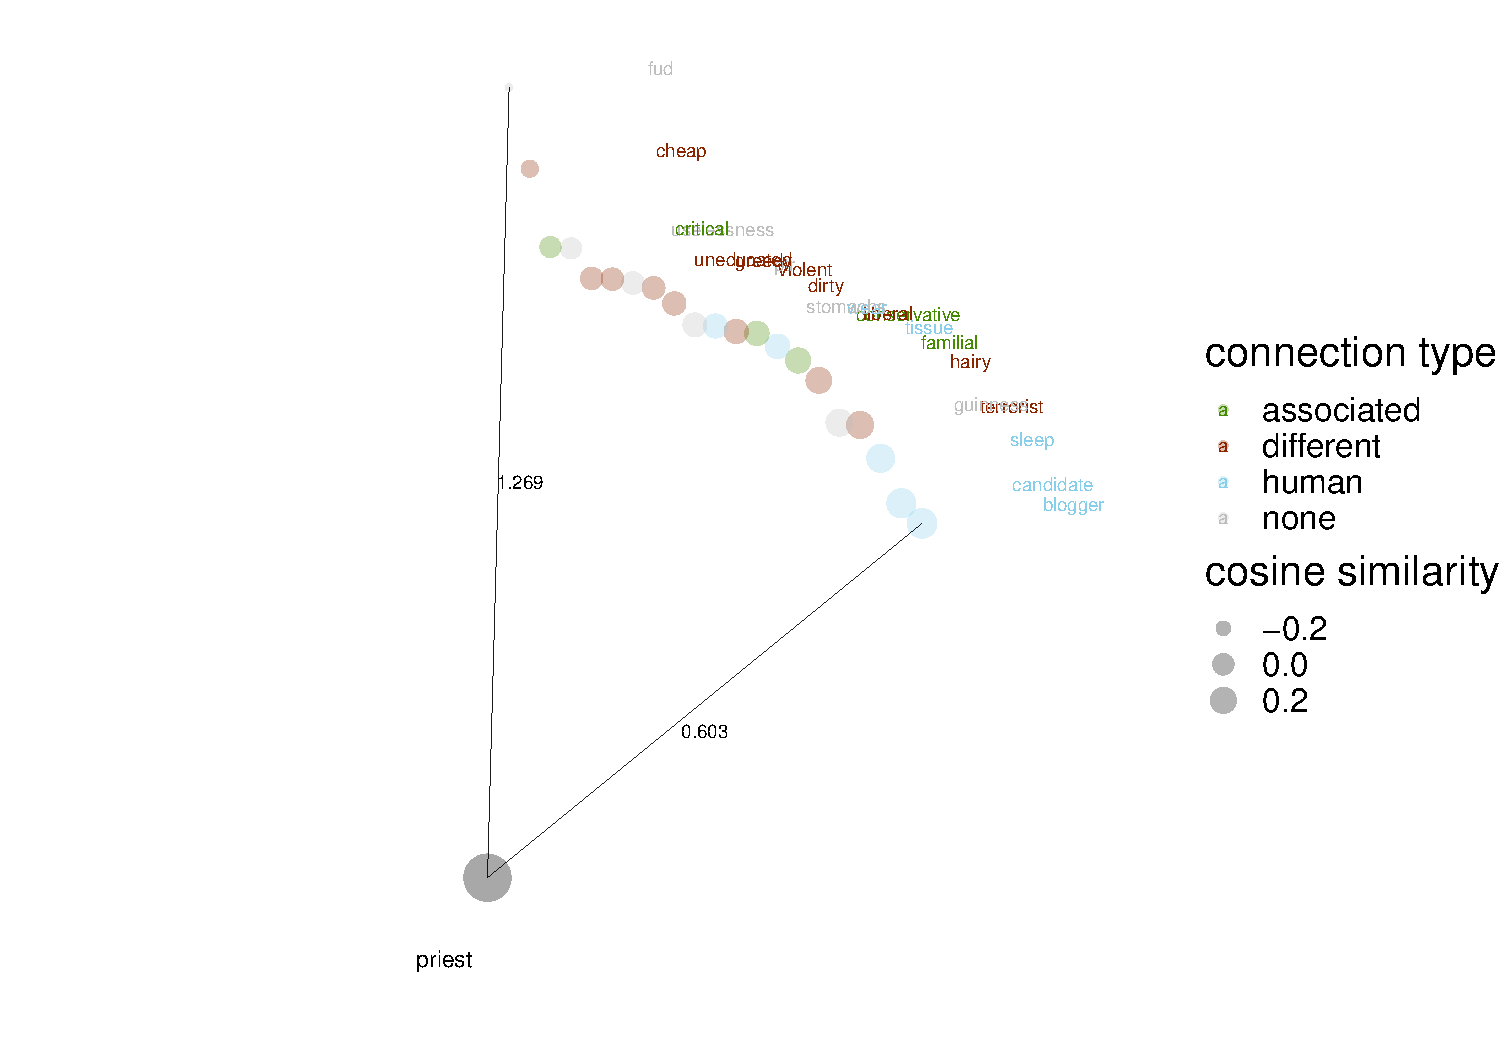
\includegraphics[width=8cm]{priest.pdf}

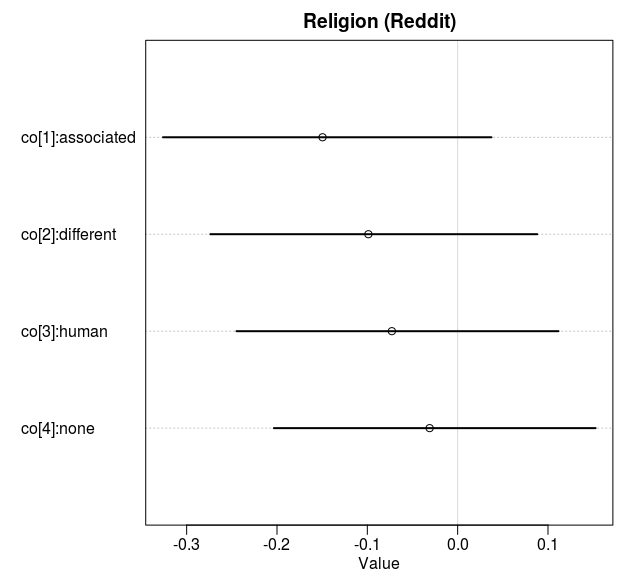
\includegraphics[width=8cm]{../images/religionCoeffs.jpeg}
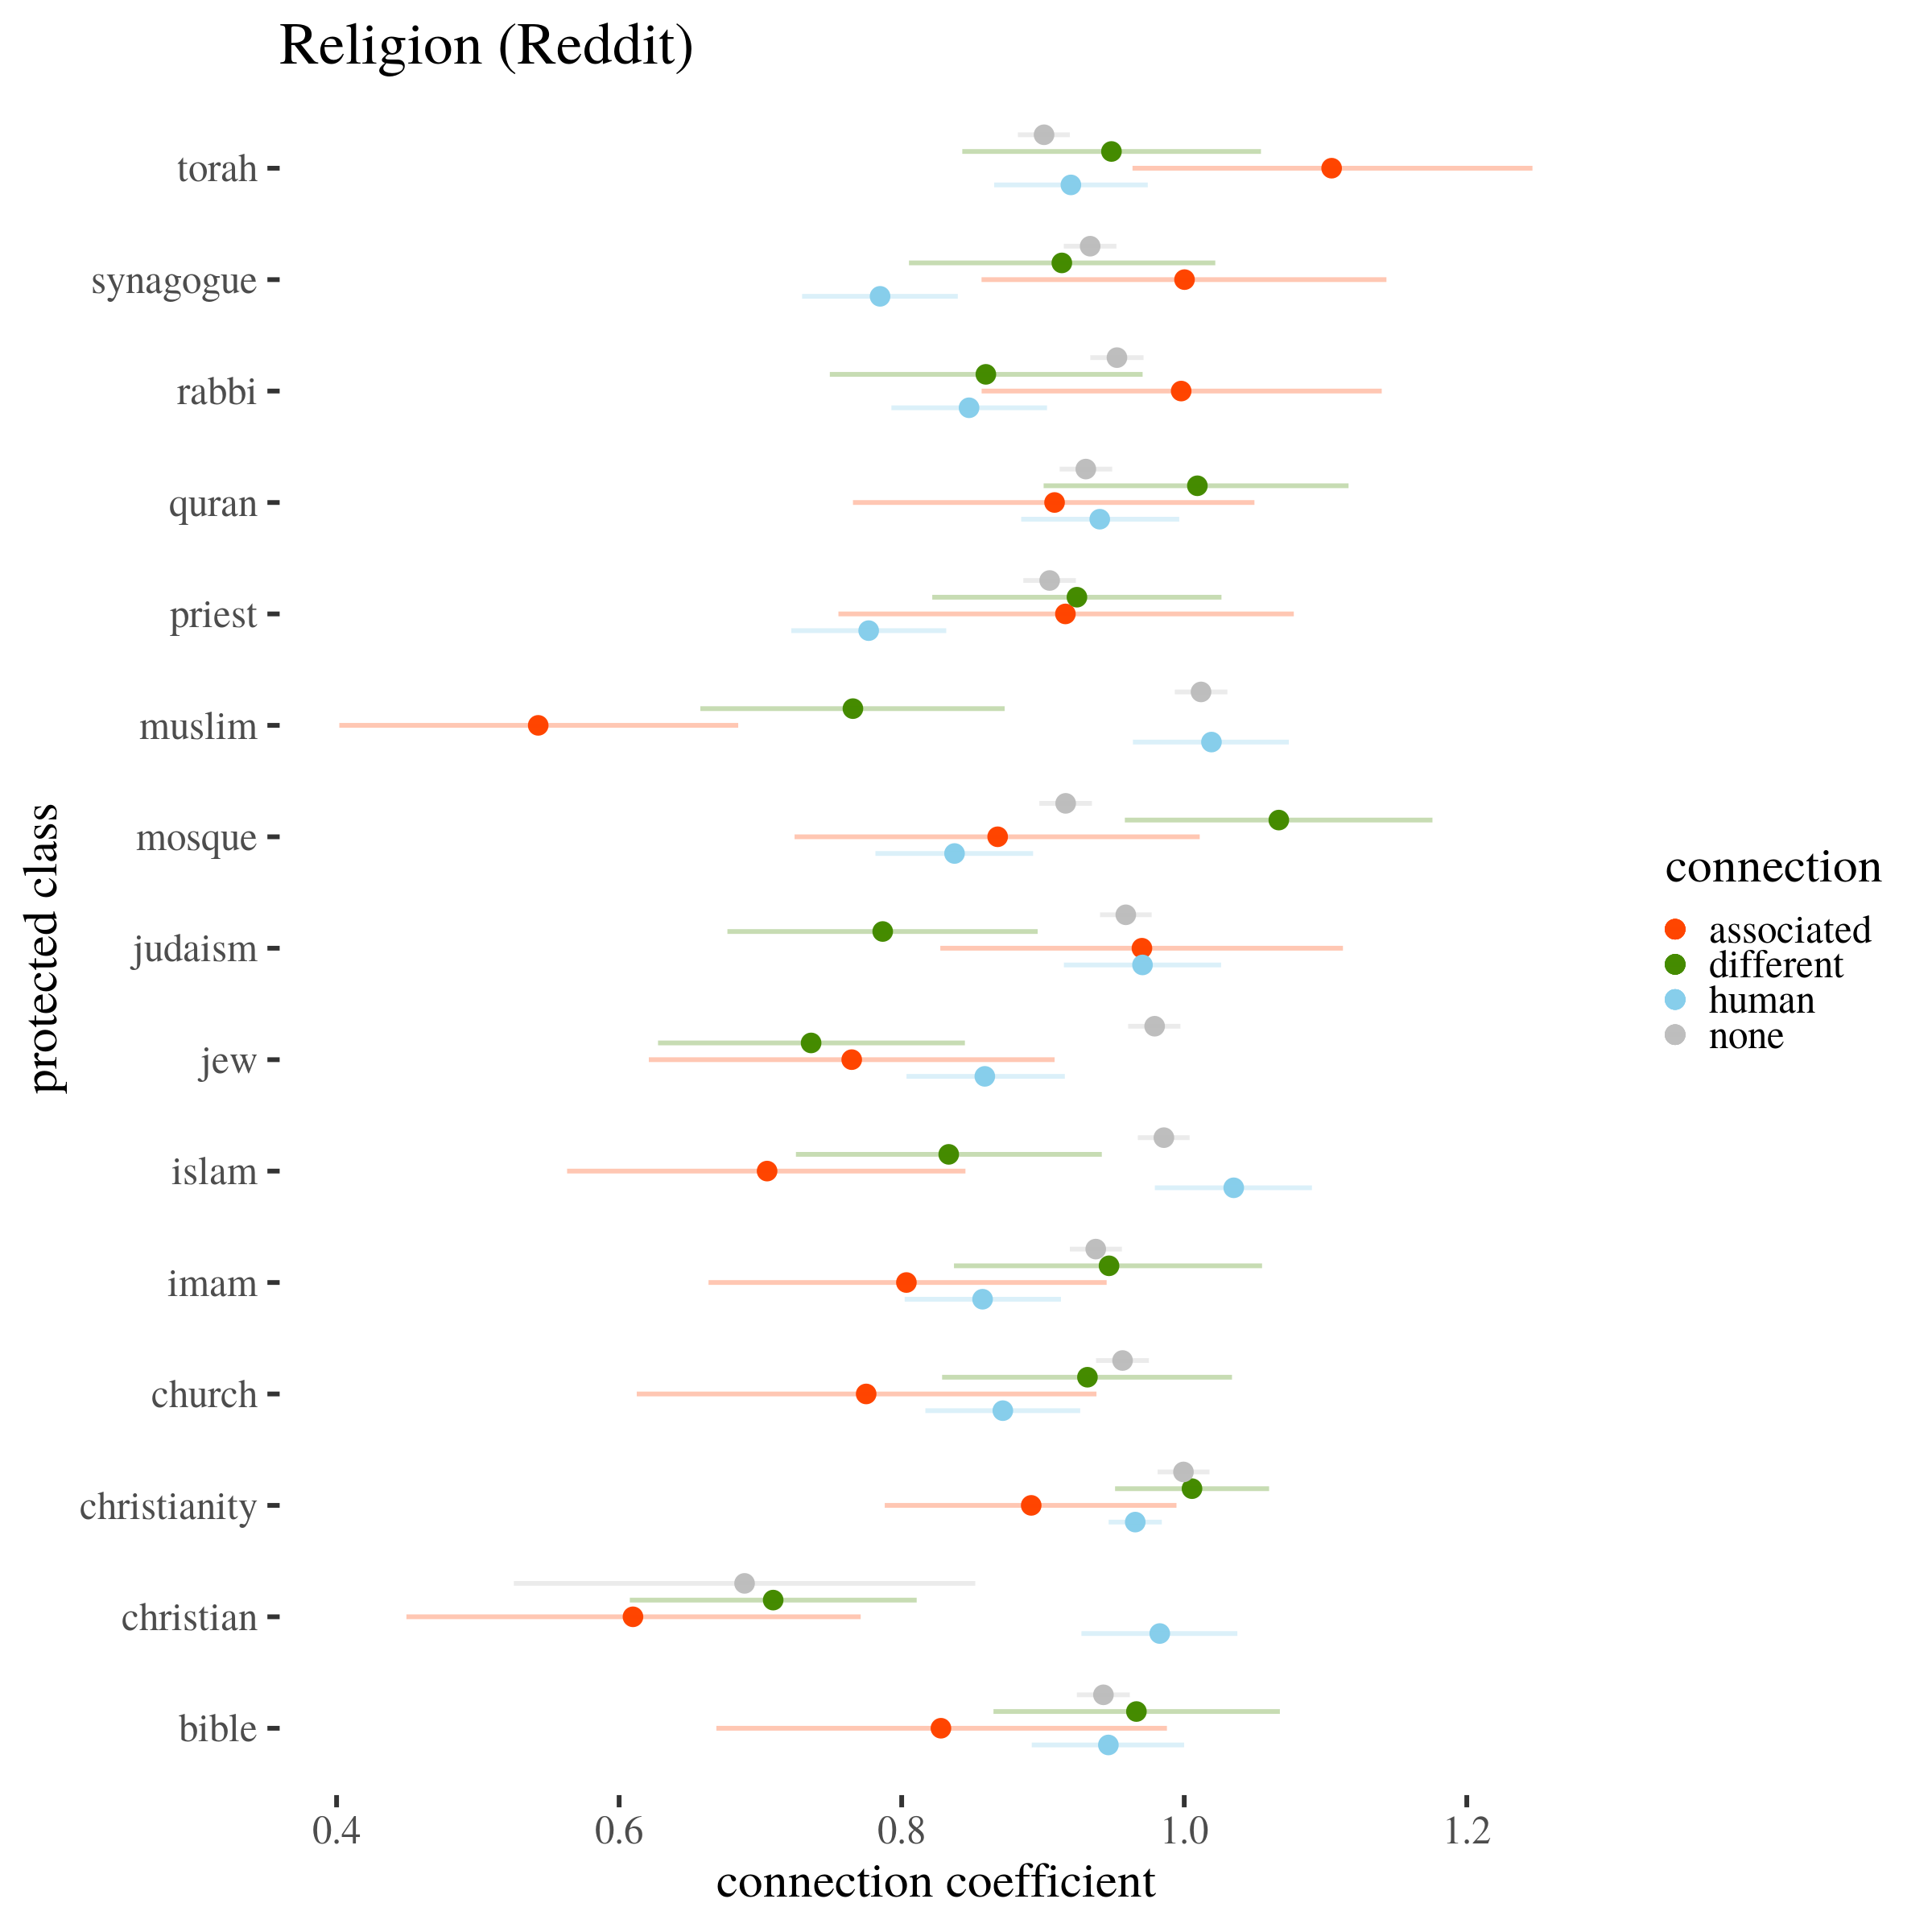
\includegraphics[width=8cm]{../images/visReligionReddit.png}

\pagebreak

\hypertarget{references}{%
\subsection*{References}\label{references}}
\addcontentsline{toc}{subsection}{References}

\scriptsize

\hypertarget{refs}{}
\begin{CSLReferences}{0}{0}
\leavevmode\hypertarget{ref-Bolukbasi2016man}{}%
\CSLLeftMargin{{[}1{]} }
\CSLRightInline{Tolga Bolukbasi, Kai-Wei Chang, James Y. Zou, Venkatesh
Saligrama, and Adam Kalai. 2016. Man is to computer programmer as woman
is to homemaker? Debiasing word embeddings. \emph{CoRR} abs/1607.06520,
(2016). Retrieved from \url{http://arxiv.org/abs/1607.06520}}

\leavevmode\hypertarget{ref-Caliskan2017semanticsBiases}{}%
\CSLLeftMargin{{[}2{]} }
\CSLRightInline{Aylin Caliskan, Joanna J. Bryson, and Arvind Narayanan.
2017. Semantics derived automatically from language corpora contain
human-like biases. \emph{Science} 356, 6334 (April 2017), 183--186.
DOI:https://doi.org/\href{https://doi.org/10.1126/science.aal4230}{10.1126/science.aal4230}}

\leavevmode\hypertarget{ref-Garg2018years}{}%
\CSLLeftMargin{{[}3{]} }
\CSLRightInline{Nikhil Garg, Londa Schiebinger, Dan Jurafsky, and James
Zou. 2018. Word embeddings quantify 100 years of gender and ethnic
stereotypes. \emph{Proceedings of the National Academy of Sciences} 115,
16 (April 2018), E3635--E3644.
DOI:https://doi.org/\href{https://doi.org/10.1073/pnas.1720347115}{10.1073/pnas.1720347115}}

\leavevmode\hypertarget{ref-Gonen2019lipstick}{}%
\CSLLeftMargin{{[}4{]} }
\CSLRightInline{Hila Gonen and Yoav Goldberg. 2019. Lipstick on a pig:
{D}ebiasing methods cover up systematic gender biases in word embeddings
but do not remove them. In \emph{Proceedings of the 2019 conference of
the north {A}merican chapter of the association for computational
linguistics: Human language technologies, volume 1 (long and short
papers)}, Association for Computational Linguistics, Minneapolis,
Minnesota, 609--614.
DOI:https://doi.org/\href{https://doi.org/10.18653/v1/N19-1061}{10.18653/v1/N19-1061}}

\leavevmode\hypertarget{ref-Lauscher2019multidimensional}{}%
\CSLLeftMargin{{[}5{]} }
\CSLRightInline{Anne Lauscher and Goran Glavas. 2019. Are we
consistently biased? Multidimensional analysis of biases in
distributional word vectors. \emph{CoRR} abs/1904.11783, (2019).
Retrieved from \url{http://arxiv.org/abs/1904.11783}}

\leavevmode\hypertarget{ref-Manzini2019blackToCriminal}{}%
\CSLLeftMargin{{[}6{]} }
\CSLRightInline{Thomas Manzini, Yao Chong Lim, Yulia Tsvetkov, and Alan
W Black. 2019. Black is to criminal as caucasian is to police: Detecting
and removing multiclass bias in word embeddings. Retrieved from
\url{http://arxiv.org/abs/1904.04047}}

\leavevmode\hypertarget{ref-Nosek2002harvesting}{}%
\CSLLeftMargin{{[}7{]} }
\CSLRightInline{Brian A. Nosek, Mahzarin R. Banaji, and Anthony G.
Greenwald. 2002. Harvesting implicit group attitudes and beliefs from a
demonstration web site. \emph{Group Dynamics: Theory, Research, and
Practice} 6, 1 (2002), 101--115.
DOI:https://doi.org/\href{https://doi.org/10.1037/1089-2699.6.1.101}{10.1037/1089-2699.6.1.101}}

\end{CSLReferences}

\end{document}
